% ============================================================
%  Reporte de práctica: Ofuscación de código en aplicaciones
%  móviles (Android / Flutter)
%  Compilar con: pdflatex reporte_ofuscacion.tex  (2 pasadas)
% ============================================================
\documentclass[12pt,letterpaper]{article}

% ---- Codificación e idioma ----
\usepackage[utf8]{inputenc}
\usepackage[T1]{fontenc}
\usepackage[spanish,es-tabla]{babel}
\usepackage{lmodern}

% ---- Página y tipografía ----
\usepackage[letterpaper,top=2.5cm,bottom=2.5cm,left=3cm,right=3cm]{geometry}
\usepackage{setspace}
\onehalfspacing
\usepackage{parskip}

% ---- Recursos ----
\usepackage{graphicx}
\usepackage{xcolor}
\usepackage{tikz}
\usetikzlibrary{arrows.meta,positioning}
\usepackage{booktabs}
\usepackage{tabularx}
\usepackage{longtable}
\usepackage{array}
\usepackage{enumitem}
\usepackage{caption}
\usepackage{listings}
\usepackage{fancyhdr}
\usepackage{titlesec}
\usepackage[hidelinks]{hyperref}

% ---- Datos editables de la portada ----
\newcommand{\alumno}{Moisés Franco Gutiérrez}
\newcommand{\matricula}{[Matrícula]}
\newcommand{\materia}{Programación para Dispositivos Móviles II}
\newcommand{\docente}{[Nombre del docente]}
\newcommand{\universidad}{[Nombre de la Universidad]}
\newcommand{\carrera}{Ingeniería en Sistemas / Desarrollo de Software}
\newcommand{\grupo}{Noveno semestre}
\newcommand{\fecha}{21 de junio de 2026}

% ---- Colores ----
\definecolor{codebg}{rgb}{0.96,0.96,0.96}
\definecolor{codekw}{rgb}{0.13,0.29,0.53}
\definecolor{codecom}{rgb}{0.30,0.55,0.30}
\definecolor{codestr}{rgb}{0.64,0.08,0.08}
\definecolor{azulinst}{rgb}{0.10,0.20,0.45}

% ---- Estilo de código (robusto ante acentos UTF-8) ----
\lstset{
  backgroundcolor=\color{codebg},
  basicstyle=\ttfamily\footnotesize,
  keywordstyle=\color{codekw}\bfseries,
  commentstyle=\color{codecom}\itshape,
  stringstyle=\color{codestr},
  numbers=left,
  numberstyle=\tiny\color{gray},
  stepnumber=1,
  breaklines=true,
  showstringspaces=false,
  frame=single,
  rulecolor=\color{gray!50},
  tabsize=2,
  captionpos=b,
  extendedchars=true,
  literate=%
    {á}{{\'a}}1 {é}{{\'e}}1 {í}{{\'i}}1 {ó}{{\'o}}1 {ú}{{\'u}}1
    {Á}{{\'A}}1 {É}{{\'E}}1 {Í}{{\'I}}1 {Ó}{{\'O}}1 {Ú}{{\'U}}1
    {ñ}{{\~n}}1 {Ñ}{{\~N}}1 {ü}{{\"u}}1 {¿}{{?`}}1 {¡}{{!`}}1
    {°}{{\textdegree}}1
}

% ---- Encabezado y pie ----
\pagestyle{fancy}
\fancyhf{}
\fancyhead[L]{\small Ofuscación de código en aplicaciones móviles}
\fancyhead[R]{\small\thepage}
\fancyfoot[C]{\small \materia}
\renewcommand{\headrulewidth}{0.4pt}

% ---- Formato de títulos ----
\titleformat{\section}{\Large\bfseries\color{azulinst}}{\thesection}{0.6em}{}
\titleformat{\subsection}{\large\bfseries\color{azulinst!85}}{\thesubsection}{0.6em}{}

% ---- Comando para marcar dónde insertar una captura de pantalla ----
\newcommand{\capturapendiente}[1]{%
  \begin{center}
  \fbox{\parbox[c][3.2cm][c]{0.85\linewidth}{\centering
    \itshape\small[\,Espacio para captura de pantalla\,]\\[4pt]#1\\[4pt]
    \footnotesize Sustituir por: \texttt{\textbackslash includegraphics[width=...]\{capturas/archivo.png\}}}}
  \end{center}
}

\begin{document}

% =====================================================================
%  PORTADA
% =====================================================================
\begin{titlepage}
\centering
\vspace*{1cm}

{\scshape\Large \universidad \par}
\vspace{0.3cm}
{\scshape \carrera \par}
\vspace{2.2cm}

\rule{\linewidth}{0.6pt}\\[0.4cm]
{\huge\bfseries Ofuscación de código en aplicaciones móviles\par}
\vspace{0.4cm}
{\Large Investigación y práctica comparativa entre una aplicación\\
\textit{con} y \textit{sin} ofuscación (Android / Flutter)\par}
\rule{\linewidth}{0.6pt}\\[1.5cm]

\begin{flushright}
\large
\begin{tabular}{rl}
\textbf{Materia:} & \materia \\[4pt]
\textbf{Alumno:} & \alumno \\[4pt]
\textbf{Matrícula:} & \matricula \\[4pt]
\textbf{Grupo:} & \grupo \\[4pt]
\textbf{Docente:} & \docente \\[4pt]
\textbf{Proyecto:} & \texttt{appmobile\_security} \\[4pt]
\end{tabular}
\end{flushright}

\vfill
{\large \fecha \par}
\end{titlepage}

% =====================================================================
%  ÍNDICE
% =====================================================================
\tableofcontents
\newpage

% =====================================================================
%  1. INTRODUCCIÓN
% =====================================================================
\section{Introducción}

Las aplicaciones móviles se distribuyen como paquetes binarios (\texttt{APK} o
\texttt{AAB}) que el usuario instala en su dispositivo. A diferencia de una
aplicación de servidor, cuyo código nunca abandona la infraestructura del
desarrollador, el binario de una aplicación móvil queda \emph{físicamente en
manos de cualquier persona} que la descargue. Esto convierte al APK en un
objetivo natural de la \textbf{ingeniería inversa}: mediante herramientas de
análisis estático y dinámico, un tercero puede recuperar parte del código
fuente, los algoritmos, las claves embebidas, las URL de los servicios y la
lógica de negocio.

Para elevar el costo de ese análisis, los desarrolladores aplican
\textbf{ofuscación de código}: un conjunto de transformaciones que conservan el
comportamiento del programa pero degradan su legibilidad. El presente documento
investiga los conceptos fundamentales de la ofuscación en Android y Flutter, y
documenta una práctica en la que se generan dos versiones de una misma
aplicación —una \emph{normal} y otra \emph{ofuscada}— para comparar, con
herramientas reales de análisis de APK, qué tan expuesta queda la lógica de
negocio en cada caso.

La aplicación utilizada es el proyecto \texttt{appmobile\_security}, desarrollado
en Flutter, que ya cumple los requisitos solicitados: contiene al menos tres
pantallas, una clase de autenticación simulada y clases que procesan información
sensible (usuario, contraseña, correo y token de sesión).

% =====================================================================
%  2. MARCO TEÓRICO
% =====================================================================
\section{Marco teórico (investigación)}

\subsection{Ingeniería inversa en aplicaciones móviles}

La \textbf{ingeniería inversa} es el proceso de analizar un producto terminado
—en este caso un binario compilado— para deducir su diseño, su funcionamiento
interno y, en la medida de lo posible, reconstruir su código fuente. En el
contexto de Android, el archivo \texttt{APK} no es más que un contenedor
\texttt{ZIP} cuyos componentes pueden extraerse y decodificarse:

\begin{itemize}[leftmargin=1.4em]
  \item \texttt{classes.dex}: el bytecode de la capa Java/Kotlin compilado para
        la máquina virtual ART/Dalvik. Es \emph{altamente} reversible: existen
        decompiladores que lo reconstruyen a un código Java muy aproximado.
  \item \texttt{resources.arsc}, \texttt{res/}: recursos, cadenas y diseños.
  \item \texttt{AndroidManifest.xml}: permisos, componentes y metadatos.
  \item \texttt{lib/}: bibliotecas nativas (\texttt{.so}) en código máquina
        (ARM/x86). En una app Flutter, aquí vive \texttt{libapp.so}, el código
        Dart compilado de forma \emph{Ahead-Of-Time} (AOT).
\end{itemize}

El flujo típico de un analista es: (1) \textbf{desempaquetar} el APK con
\texttt{apktool}; (2) \textbf{decompilar} el \texttt{.dex} con \texttt{JADX} o
\texttt{Bytecode Viewer} para leer el código Java reconstruido; (3) opcionalmente
\textbf{instrumentar} la app en ejecución con herramientas dinámicas (Frida,
Objection) para observar valores en tiempo real. La ingeniería inversa es además
una técnica \emph{legítima} en auditorías de seguridad, análisis de malware e
interoperabilidad; el problema surge cuando se emplea para robar propiedad
intelectual o atacar a los usuarios.

\subsection{Riesgos de seguridad asociados a la exposición del código fuente}

Cuando el código de una aplicación queda expuesto, los riesgos más relevantes
son:

\begin{itemize}[leftmargin=1.4em]
  \item \textbf{Robo de secretos embebidos}: claves de API, tokens, contraseñas
        o certificados escritos directamente en el código (\emph{hardcoded}).
  \item \textbf{Descubrimiento de endpoints}: URL de servicios internos, rutas y
        parámetros que facilitan atacar el \emph{backend}.
  \item \textbf{Evasión de controles del lado cliente}: validaciones, límites de
        prueba, comprobaciones de licencia o de seguridad que un atacante puede
        identificar y desactivar.
  \item \textbf{Robo de propiedad intelectual}: algoritmos propietarios y lógica
        de negocio que constituyen una ventaja competitiva.
  \item \textbf{\emph{Repackaging} / troyanización}: modificar la app, reinsertar
        código malicioso y redistribuirla suplantando a la original.
  \item \textbf{Identificación de vulnerabilidades}: leer el código facilita
        encontrar fallos explotables.
\end{itemize}

\subsection{Concepto de ofuscación de código}

La \textbf{ofuscación} es la transformación deliberada de un programa para que
sea difícil de entender por un humano (y por herramientas automáticas),
\emph{sin alterar su comportamiento observable}. El programa ofuscado se ejecuta
exactamente igual que el original, pero su código —nombres, estructura, flujo—
deja de ser informativo. Es importante subrayar que la ofuscación \textbf{no es
cifrado}: el código no se vuelve ilegible para la máquina, solo para el analista;
sigue presente y ejecutable.

\subsection{Diferencias: ofuscación, minimización, optimización y cifrado}

Estos cuatro términos suelen confundirse, pero persiguen objetivos distintos.
La tabla~\ref{tab:conceptos} los contrasta.

\begin{table}[h]
\centering
\caption{Diferencias entre ofuscación, minimización, optimización y cifrado.}
\label{tab:conceptos}
\renewcommand{\arraystretch}{1.3}
\begin{tabularx}{\linewidth}{>{\bfseries}l X l}
\toprule
Técnica & Qué hace & Objetivo \\
\midrule
Ofuscación & Renombra identificadores y altera la estructura/flujo para que el código sea difícil de comprender. & Confidencialidad / dificultar el análisis. \\
Minimización (\emph{Shrinking}) & Elimina clases, métodos, campos y recursos que no se usan (\emph{tree-shaking}). & Reducir el tamaño del binario. \\
Optimización & Reescribe el código para que sea más eficiente o compacto (\emph{inlining}, eliminación de código muerto, fusión de clases). & Rendimiento y tamaño. \\
Cifrado de código & Almacena clases/cadenas cifradas y las descifra en tiempo de ejecución (\emph{packers}, \emph{string encryption}). & Protección fuerte del contenido. \\
\bottomrule
\end{tabularx}
\end{table}

La diferencia clave: la \textbf{minimización} y la \textbf{optimización} buscan
principalmente \emph{eficiencia} (aunque como efecto secundario dificultan la
lectura), mientras que la \textbf{ofuscación} busca explícitamente
\emph{ocultar}. El \textbf{cifrado} es la protección más fuerte, pero conlleva
una contradicción fundamental: para ejecutarse, la app debe descifrar el código,
de modo que la clave de descifrado vive dentro del propio binario y puede
extraerse mediante análisis dinámico. Herramientas como \textbf{R8} combinan
shrinking + optimización + ofuscación en una sola pasada; el cifrado pertenece a
soluciones comerciales como \textbf{DexGuard}.

\subsection{Herramientas de ofuscación en Android: ProGuard y R8}

\paragraph{ProGuard.} Fue durante años la herramienta estándar (de la empresa
Guardsquare). Realiza cuatro fases: \emph{shrink} (elimina código no usado),
\emph{optimize}, \emph{obfuscate} (renombra) y \emph{preverify}. Se configura
con un archivo de reglas (\texttt{proguard-rules.pro}) basado en directivas
\texttt{-keep}.

\paragraph{R8.} Es el compilador/ofuscador \emph{oficial} de Google, integrado en
el \emph{Android Gradle Plugin} desde la versión 3.4 y activado por defecto en
lugar de ProGuard. R8 hace en un solo paso el \emph{shrinking}, el
\emph{desugaring}, la optimización y la ofuscación, es más rápido y produce
binarios más pequeños. Mantiene compatibilidad con la sintaxis de reglas de
ProGuard, por lo que el mismo \texttt{proguard-rules.pro} sirve para ambos. Se
activa estableciendo \texttt{isMinifyEnabled = true} en el bloque \texttt{release}
de Gradle. La versión comercial, \textbf{DexGuard}, añade cifrado de cadenas y
clases, ofuscación de flujo de control y protecciones en tiempo de ejecución
(RASP).

\subsection{Mecanismos de ofuscación en Flutter}

Una aplicación Flutter tiene \emph{dos capas} de código que se ofuscan de forma
independiente:

\begin{enumerate}[leftmargin=1.6em]
  \item \textbf{Capa nativa de host (Java/Kotlin)}: el \emph{embedding} de
        Android, los \emph{plugins} y el \texttt{MainActivity}. Se ofusca con
        \textbf{R8/ProGuard}, igual que cualquier app Android.
  \item \textbf{Capa Dart}: en una compilación \emph{release}, el código Dart se
        compila AOT a código máquina dentro de \texttt{libapp.so}. Aun así, los
        nombres de funciones y clases pueden quedar como símbolos legibles. Para
        ocultarlos se usa la bandera de compilación:
\begin{lstlisting}[language=bash]
flutter build apk --release --obfuscate --split-debug-info=build/symbols
\end{lstlisting}
        La opción \texttt{--obfuscate} reemplaza los nombres de los símbolos Dart
        por identificadores sin sentido, y \texttt{--split-debug-info} extrae un
        \emph{mapa de símbolos} a la carpeta indicada. Ese mapa es indispensable
        para \emph{des-ofuscar} los \emph{stack traces} de producción con
        \texttt{flutter symbolize}; sin él, los reportes de error son ilegibles.
\end{enumerate}

Conviene notar que el código Dart compilado a AOT ya es, de partida, más difícil
de revertir que el bytecode DEX, porque es código máquina nativo y no bytecode
de alto nivel. La ofuscación de Flutter refuerza esa barrera ocultando los
símbolos restantes.

\subsection{Tipos de técnicas de ofuscación}

\begin{itemize}[leftmargin=1.4em]
  \item \textbf{Renombrado de clases}: \texttt{LoginViewModel} pasa a llamarse
        \texttt{a}, \texttt{SecureSessionStore} a \texttt{b}, etc. Se pierde toda
        pista semántica del propósito de la clase.
  \item \textbf{Renombrado de métodos}: \texttt{validatePassword()} se convierte
        en \texttt{a()}; \texttt{saveSensitiveFields()} en \texttt{b()}.
  \item \textbf{Renombrado de variables y campos}: \texttt{sessionToken} pasa a
        \texttt{c}, \texttt{\_currentUser} a \texttt{d}.
  \item \textbf{Eliminación de código no utilizado} (\emph{shrinking}): se borran
        las clases, métodos y recursos que el analizador determina inalcanzables;
        además de reducir el tamaño, deja menos código que estudiar.
  \item \textbf{Ofuscación del flujo de control} (\emph{Control Flow
        Obfuscation}): se reescribe el grafo de ejecución insertando saltos,
        \emph{predicados opacos} y aplanamiento de estructuras (\emph{control flow
        flattening}) para que el flujo lógico sea difícil de seguir. R8 no la
        aplica de forma agresiva; es propia de herramientas comerciales como
        DexGuard.
\end{itemize}

\subsection{Ventajas y desventajas de la ofuscación}

\begin{table}[h]
\centering
\caption{Ventajas y desventajas de la ofuscación.}
\label{tab:ventajas}
\renewcommand{\arraystretch}{1.25}
\begin{tabularx}{\linewidth}{X X}
\toprule
\textbf{Ventajas} & \textbf{Desventajas} \\
\midrule
Eleva el costo y el tiempo de la ingeniería inversa. & No la impide: solo la encarece (no es una barrera absoluta). \\
Oculta nombres y lógica, protegiendo la propiedad intelectual. & Dificulta la depuración: se requiere el mapa de símbolos/\emph{mapping} para leer los \emph{stack traces}. \\
El \emph{shrinking} reduce el tamaño del APK. & Puede romper reflexión, serialización o JNI si faltan reglas \texttt{-keep}. \\
Activación sencilla (una bandera en Gradle / Flutter). & Aumenta el mantenimiento: hay que conservar reglas \emph{keep} y mapas por versión. \\
Mejora marginal de rendimiento por la optimización. & Genera una \emph{falsa sensación de seguridad} si se usa como única defensa. \\
\bottomrule
\end{tabularx}
\end{table}

\subsection{Casos donde la ofuscación afecta a bibliotecas de terceros}

La ofuscación puede \textbf{romper} el funcionamiento de bibliotecas que dependen
del \emph{nombre} de las clases o de los miembros en tiempo de ejecución:

\begin{itemize}[leftmargin=1.4em]
  \item \textbf{Reflexión}: librerías como Gson, Jackson o Retrofit acceden a
        campos por su nombre; si R8 los renombra, la (de)serialización falla.
  \item \textbf{JNI / código nativo}: los métodos \texttt{native} se resuelven
        por nombre desde el código C/C++; renombrarlos provoca
        \texttt{UnsatisfiedLinkError}. En Flutter esto aplica al \emph{engine} y
        a los plugins.
  \item \textbf{Frameworks que cargan clases dinámicamente} (Firebase, inyección
        de dependencias) esperan nombres concretos.
\end{itemize}

La solución son las reglas \texttt{-keep}, que indican a R8 qué no debe tocar.
Muchas librerías ya incluyen sus propias reglas (\texttt{consumer-rules.pro}),
pero el desarrollador debe añadir las suyas para los modelos de datos y las
clases accedidas por reflexión. En este proyecto fue necesario conservar
\texttt{io.flutter.**}, \texttt{com.google.firebase.**}, los métodos nativos y
\texttt{androidx.security.crypto.**} (usado por \texttt{flutter\_secure\_storage}).

\subsection{Buenas prácticas para proteger aplicaciones móviles}

\begin{enumerate}[leftmargin=1.6em]
  \item \textbf{No almacenar secretos en el cliente}: las claves de API y los
        secretos deben vivir en el \emph{backend}; el cliente solo debe recibir
        tokens de corta duración.
  \item \textbf{Ofuscación + \emph{shrinking}} en \emph{release}, tanto en la capa
        Dart como en la capa Java/Kotlin.
  \item \textbf{Almacenamiento seguro}: usar Android Keystore / iOS Keychain y
        \texttt{EncryptedSharedPreferences} (como hace este proyecto con
        \texttt{flutter\_secure\_storage}).
  \item \textbf{Cifrado de cadenas sensibles} y, en apps críticas, cifrado de
        código (DexGuard u otros).
  \item \textbf{Comunicaciones seguras}: TLS y \emph{certificate pinning}.
  \item \textbf{Validación del lado servidor}: nunca confiar en validaciones que
        ocurren solo en el cliente.
  \item \textbf{Anti-\emph{tampering} y RASP}: detección de \emph{root},
        emulador, depuración (USB) y \emph{hooking}; verificación de integridad y
        de firma; uso de la \emph{Play Integrity API}.
  \item \textbf{Defensa en profundidad}: combinar varias medidas, asumiendo que
        cualquiera puede ser vulnerada por separado.
\end{enumerate}

% =====================================================================
%  3. DESARROLLO DE LA PRÁCTICA
% =====================================================================
\section{Desarrollo de la práctica}

\subsection{Descripción de la aplicación}

El proyecto \texttt{appmobile\_security} (Flutter) cumple los requisitos de la
práctica:

\begin{itemize}[leftmargin=1.4em]
  \item \textbf{Tres pantallas}: \texttt{LoginView} (inicio de sesión),
        \texttt{RegisterView} (registro) y \texttt{HomeView} (panel con datos de
        sesión).
  \item \textbf{Clase de autenticación simulada}: \texttt{FakeAuthRepository},
        que valida credenciales contra una lista local de usuarios y genera un
        token de sesión.
  \item \textbf{Clases que procesan información sensible}:
        \texttt{SecureSessionStore} y \texttt{SessionManager}, que guardan y leen
        usuario, contraseña, correo y token de sesión en el almacén cifrado del
        sistema operativo.
\end{itemize}

La figura~\ref{fig:arq} resume la arquitectura: las tres pantallas se apoyan en
la clase de autenticación simulada, que a su vez entrega el token al gestor de
sesión y a la capa de almacenamiento cifrado.

\begin{figure}[h]
\centering
\begin{tikzpicture}[
  font=\footnotesize,
  scr/.style={rectangle, rounded corners, draw=blue!60, thick, fill=blue!8,
              align=center, minimum height=0.9cm, minimum width=2.5cm},
  auth/.style={rectangle, rounded corners, draw=orange!75, thick, fill=orange!12,
               align=center, minimum height=1.0cm, minimum width=8.2cm},
  data/.style={rectangle, rounded corners, draw=teal!75, thick, fill=teal!10,
               align=center, minimum height=1.0cm, minimum width=8.2cm},
  store/.style={rectangle, rounded corners, draw=gray!75, thick, fill=gray!15,
                align=center, minimum height=1.0cm, minimum width=8.2cm},
  arr/.style={-{Latex[length=2.4mm]}, thick}
]
\node[scr] (register) {RegisterView};
\node[scr, left=0.5cm of register]  (login) {LoginView};
\node[scr, right=0.5cm of register] (home)  {HomeView};
\node[font=\bfseries\scriptsize, above=0.1cm of register] {Pantallas (UI)};
\node[auth,  below=1.2cm of register] (auth) {\textbf{FakeAuthRepository} -- autenticación simulada\\\scriptsize login() \quad register() \quad \_generateToken()};
\node[data,  below=0.8cm of auth] (sm) {\textbf{SessionManager} -- orquesta la sesión\\\scriptsize startSession() \quad readSensitiveFields()};
\node[data,  below=0.8cm of sm]  (ss) {\textbf{SecureSessionStore} -- procesa datos sensibles\\\scriptsize saveSensitiveFields() / readSensitiveFields()};
\node[store, below=0.8cm of ss]  (enc) {\textbf{Almacén cifrado del SO}\\\scriptsize EncryptedSharedPreferences (Android) / Keychain (iOS)};
\draw[arr] (login)    -- (auth);
\draw[arr] (register) -- (auth);
\draw[arr] (home)     -- (sm);
\draw[arr] (auth) -- node[right, font=\scriptsize] {token} (sm);
\draw[arr] (sm)   -- (ss);
\draw[arr] (ss)   -- node[right, font=\scriptsize] {usuario, contraseña, correo, token} (enc);
\end{tikzpicture}
\caption{Arquitectura de la aplicación: las tres pantallas, la clase de autenticación simulada y las clases que procesan y almacenan la información sensible.}
\label{fig:arq}
\end{figure}

A modo de ejemplo, el fragmento~\ref{lst:auth} muestra la lógica de negocio que
\emph{queremos proteger}: la generación del token y la validación de
credenciales. Tras la ofuscación, los nombres \texttt{FakeAuthRepository},
\texttt{login} o \texttt{\_generateToken} dejan de ser visibles en la capa
correspondiente.

\begin{lstlisting}[language=Java,caption={Lógica de negocio sensible (clase de autenticación simulada, en Dart).},label=lst:auth]
class FakeAuthRepository {
  // ... usuario demo y token de sesión ...
  Future<AppUser> login({required String email, required String password}) async {
    // valida credenciales y genera el token de sesión
  }
  String _generateToken() {
    final Random random = Random.secure();
    final List<int> bytes = List<int>.generate(24, (_) => random.nextInt(256));
    return 'sess_${base64Url.encode(bytes).replaceAll('=', '')}';
  }
}
\end{lstlisting}

\subsection{Configuración aplicada para la ofuscación}

Se modificó el bloque \texttt{release} de
\texttt{android/app/build.gradle.kts} para activar R8 de forma
\emph{condicional}. La configuración detecta la propiedad
\texttt{dart-obfuscation}, que Flutter envía a Gradle cuando se compila con
\texttt{--obfuscate}; además conserva \texttt{obfuscate} como interruptor manual.
Así se generan ambas versiones desde el mismo proyecto sin editar el archivo
entre compilaciones (fragmento~\ref{lst:gradle}).

\begin{lstlisting}[language=Java,caption={Activación condicional de R8 en \texttt{build.gradle.kts}.},label=lst:gradle]
buildTypes {
    release {
        signingConfig = signingConfigs.getByName("debug")

        // R8 se activa cuando Flutter compila con --obfuscate
        fun flag(name: String) =
            (project.findProperty(name) as String?)?.toBoolean() ?: false
        val enableObfuscation = flag("dart-obfuscation") || flag("obfuscate")

        isMinifyEnabled = enableObfuscation     // activa R8 (shrink + ofuscacion)
        isShrinkResources = enableObfuscation   // elimina recursos no usados

        proguardFiles(
            getDefaultProguardFile("proguard-android-optimize.txt"),
            "proguard-rules.pro",
        )
    }
}
\end{lstlisting}

El archivo \texttt{android/app/proguard-rules.pro} contiene las reglas
\texttt{-keep} que evitan que R8 rompa Flutter, Firebase, los métodos nativos y
el almacenamiento seguro (fragmento~\ref{lst:proguard}).

\begin{lstlisting}[caption={Extracto de \texttt{proguard-rules.pro}.},label=lst:proguard]
# Motor y plugins de Flutter (reflexion + JNI)
-keep class io.flutter.** { *; }
-keep class io.flutter.plugins.** { *; }

# Metodos nativos (JNI): no renombrar
-keepclasseswithmembernames class * { native <methods>; }

# Firebase / Google Play Services
-keep class com.google.firebase.** { *; }
-keep class com.google.android.gms.** { *; }

# flutter_secure_storage / EncryptedSharedPreferences
-keep class androidx.security.crypto.** { *; }

# Conserva numeros de linea pero oculta el nombre del archivo fuente
-keepattributes SourceFile,LineNumberTable
-renamesourcefileattribute SourceFile
\end{lstlisting}

\subsection{Generación de la versión normal (sin ofuscar)}

\begin{lstlisting}[language=bash]
flutter clean
flutter build apk --release
# Salida: build/app/outputs/flutter-apk/app-release.apk
\end{lstlisting}

Al no pasar \texttt{--obfuscate} ni definir \texttt{obfuscate=true},
\texttt{isMinifyEnabled} queda en \texttt{false}: R8 no se ejecuta y los nombres
de la capa Java/Kotlin permanecen intactos. Tampoco se ofuscan los símbolos Dart.

\subsection{Generación de la versión ofuscada}

\begin{lstlisting}[language=bash]
# PowerShell (Windows)
flutter build apk --release --obfuscate --split-debug-info=build/symbols

# Bash (Linux/macOS)
flutter build apk --release --obfuscate --split-debug-info=build/symbols

# Alternativa manual para forzar R8 sin ofuscar Dart:
$env:ORG_GRADLE_PROJECT_obfuscate="true"   # PowerShell
flutter build apk --release
$env:ORG_GRADLE_PROJECT_obfuscate=$null
\end{lstlisting}

Aquí se activan simultáneamente las dos capas de ofuscación: R8 (capa
Java/Kotlin, vía la propiedad de Gradle \texttt{dart-obfuscation}) y
\texttt{--obfuscate} (capa Dart). El mapa de símbolos queda en
\texttt{build/symbols} para des-ofuscar \emph{stack traces}.

\subsection{Herramientas de análisis utilizadas}

\begin{itemize}[leftmargin=1.4em]
  \item \textbf{JADX}: decompila \texttt{classes.dex} a código Java legible.
        Permite comparar directamente los nombres de clases y métodos.
  \item \textbf{APKTool}: desempaqueta el APK, decodifica el
        \texttt{AndroidManifest.xml}, los recursos y desensambla a
        \emph{smali}. Útil para ver la estructura y el número de clases.
  \item \textbf{Bytecode Viewer}: entorno gráfico que integra varios
        decompiladores (CFR, Procyon, Fernflower) y el desensamblador smali en
        una sola vista.
\end{itemize}

% =====================================================================
%  4. RESULTADOS Y COMPARACIÓN
% =====================================================================
\section{Resultados y comparación}

\subsection{Tabla comparativa de resultados}

La tabla~\ref{tab:comparativa} resume la comparación entre ambas versiones.
Las cifras de tamaño y de número de clases provienen de la compilación y del
análisis realizados en este equipo (ver capturas).

\begin{table}[h]
\centering
\caption{Comparación entre la APK normal y la APK ofuscada.}
\label{tab:comparativa}
\renewcommand{\arraystretch}{1.35}
\begin{tabularx}{\linewidth}{>{\bfseries}p{4.5cm} X X}
\toprule
Criterio & APK normal & APK ofuscada \\
\midrule
Tamaño del APK & 53.28 MB & 46.65 MB ($-6.63$ MB, $\approx 12.4\%$) \\
Minificación R8 / \emph{shrink} & Desactivada & Activada \\
Ofuscación de Dart & No & Sí (\texttt{--obfuscate}) \\
Archivos \texttt{.dex} & 2 archivos (12.80 MB) & 1 archivo (2.57 MB, $\approx 80\%$ menos) \\
Clases (medidas con JADX) & 3\,529 & 1\,587 ($\approx 55\%$ menos) \\
Archivo \texttt{mapping.txt} (R8) & No se genera & 124\,011 líneas, 3\,559 clases \\
Nombres de clases & Descriptivos & Renombrados (\texttt{a.a}, \texttt{b.q}, \texttt{p2.d}\ldots) \\
Nombres de métodos y campos & Descriptivos & Renombrados (\texttt{a()}, \texttt{b}\ldots) \\
Símbolos Dart en \texttt{libapp.so} & Visibles (\texttt{grep}) & Ocultos \\
Facilidad para comprender la lógica & Alta & Baja \\
\bottomrule
\end{tabularx}
\end{table}

La figura~\ref{fig:barras} muestra esos mismos datos de forma visual.

\begin{figure}[h]
\centering
\begin{tikzpicture}[font=\footnotesize]
  % --- Tamaño del APK ---
  \node[anchor=east] at (-0.15,4.0) {Tamaño APK};
  \fill[blue!45] (0,3.85) rectangle (6.00,4.15);
  \node[anchor=west,font=\scriptsize] at (6.05,4.0) {53.28 MB};
  \fill[teal!55] (0,3.45) rectangle (5.25,3.75);
  \node[anchor=west,font=\scriptsize] at (5.30,3.6) {46.65 MB};
  % --- Bytecode .dex ---
  \node[anchor=east] at (-0.15,2.9) {Bytecode .dex};
  \fill[blue!45] (0,2.75) rectangle (6.00,3.05);
  \node[anchor=west,font=\scriptsize] at (6.05,2.9) {12.80 MB (2 dex)};
  \fill[teal!55] (0,2.35) rectangle (1.20,2.65);
  \node[anchor=west,font=\scriptsize] at (1.25,2.5) {2.57 MB (1 dex)};
  % --- Clases ---
  \node[anchor=east] at (-0.15,1.8) {Clases (JADX)};
  \fill[blue!45] (0,1.65) rectangle (6.00,1.95);
  \node[anchor=west,font=\scriptsize] at (6.05,1.8) {3\,529};
  \fill[teal!55] (0,1.25) rectangle (2.70,1.55);
  \node[anchor=west,font=\scriptsize] at (2.75,1.4) {1\,587};
  % --- Leyenda ---
  \fill[blue!45] (0,0.5) rectangle (0.4,0.8);
  \node[anchor=west] at (0.45,0.65) {Normal};
  \fill[teal!55] (2.0,0.5) rectangle (2.4,0.8);
  \node[anchor=west] at (2.45,0.65) {Ofuscada};
\end{tikzpicture}
\caption{Comparación visual normal vs.\ ofuscada. Las barras son proporcionales
al valor de la versión normal; cuanto más corta la barra ofuscada (teal), mayor
es el efecto del \emph{shrinking} y la ofuscación de R8.}
\label{fig:barras}
\end{figure}

\subsection{Comparación de nombres de clases (JADX)}

Al abrir ambos APK en JADX se observa el contraste directo. En la versión
\textbf{normal}, la jerarquía de paquetes y los nombres son descriptivos; en la
\textbf{ofuscada}, R8 colapsa los nombres a uno o dos caracteres y aplana la
jerarquía (la APK ofuscada contiene más de cien paquetes de 1--2 letras:
\texttt{a/}, \texttt{b/}, \ldots, \texttt{p2/}, \texttt{q2/}, \texttt{z2/}). El
fragmento~\ref{lst:jadx} muestra correspondencias \emph{reales} tomadas del
\texttt{mapping.txt} generado por R8 en esta práctica.

\begin{lstlisting}[caption={Correspondencias reales de nombres (\texttt{mapping.txt} de R8).},label=lst:jadx]
== CLASES RENOMBRADAS (ofuscadas) ==
com.it_nomads.fluttersecurestorage.FlutterSecureStoragePlugin          -> p2.d
com.it_nomads.fluttersecurestorage.ciphers.RSACipherOAEPImplementation -> q2.b
androidx.activity.ComponentActivity                                    -> b.q
_COROUTINE._BOUNDARY                                                   -> a.a

== CLASES CONSERVADAS por reglas -keep / manifiesto (sin cambio) ==
com.example.appmobile_security.MainActivity      -> (igual)   # entrada del manifiesto
io.flutter.embedding.android.FlutterActivity     -> (igual)   # -keep io.flutter.**
com.google.firebase.messaging.FirebaseMessaging  -> (igual)   # -keep firebase
\end{lstlisting}

\textit{Nota: el \texttt{MainActivity}, las clases \texttt{io.flutter.**} y
Firebase se conservan porque las reglas \texttt{-keep} (y el manifiesto) se lo
indican a R8; lo que se ofusca es el resto del código y las dependencias no
protegidas, como el \emph{plugin} de almacenamiento seguro
(\texttt{com.it\_nomads\ldots} $\rightarrow$ \texttt{p2.d}).}

\subsection{Símbolos Dart en la biblioteca nativa (\texttt{libapp.so})}

La lógica de negocio de la aplicación (la clase de autenticación
\texttt{FakeAuthRepository} y las clases que procesan datos sensibles
\texttt{SessionManager} y \texttt{SecureSessionStore}) no vive en el
\texttt{.dex}, sino compilada AOT dentro de \texttt{lib/arm64-v8a/libapp.so}.
Para comprobar el efecto de \texttt{--obfuscate} se buscaron, con una simple
orden \texttt{grep}, los nombres de esas clases y métodos dentro del binario de
cada versión. El resultado (tabla~\ref{tab:symbols}) es contundente.

\begin{table}[h]
\centering
\caption{Coincidencias de símbolos Dart de la app en \texttt{libapp.so} (arm64).}
\label{tab:symbols}
\renewcommand{\arraystretch}{1.2}
\begin{tabularx}{\linewidth}{>{\ttfamily}X c c}
\toprule
\normalfont Símbolo buscado & APK normal & APK ofuscada \\
\midrule
FakeAuthRepository  & 2 & 0 \\
SessionManager      & 2 & 0 \\
SecureSessionStore  & 1 & 0 \\
\_generateToken     & 1 & 0 \\
saveSensitiveFields & 1 & 0 \\
\bottomrule
\end{tabularx}
\end{table}

En la versión \textbf{normal}, el nombre de la clase de autenticación, el de la
clase que procesa los datos sensibles y el del método que genera el token son
recuperables del binario con un simple \texttt{grep}; en la versión
\textbf{ofuscada} desaparecen por completo (0 coincidencias). Esto evidencia el
valor de \texttt{--obfuscate} para ocultar la \emph{estructura} del código Dart,
aunque —como se discute en las conclusiones— no protege los \emph{valores}
constantes (cadenas, claves) que pudieran estar embebidos.

\subsection{Capturas de pantalla}

Las siguientes capturas documentan la configuración aplicada y los resultados
observados durante la práctica. Se generaron a partir de los archivos locales de
la entrega: configuración Gradle, salidas de análisis en \texttt{analisis/} y
mediciones reales de los APK incluidos.

\begin{figure}[htbp]
\centering
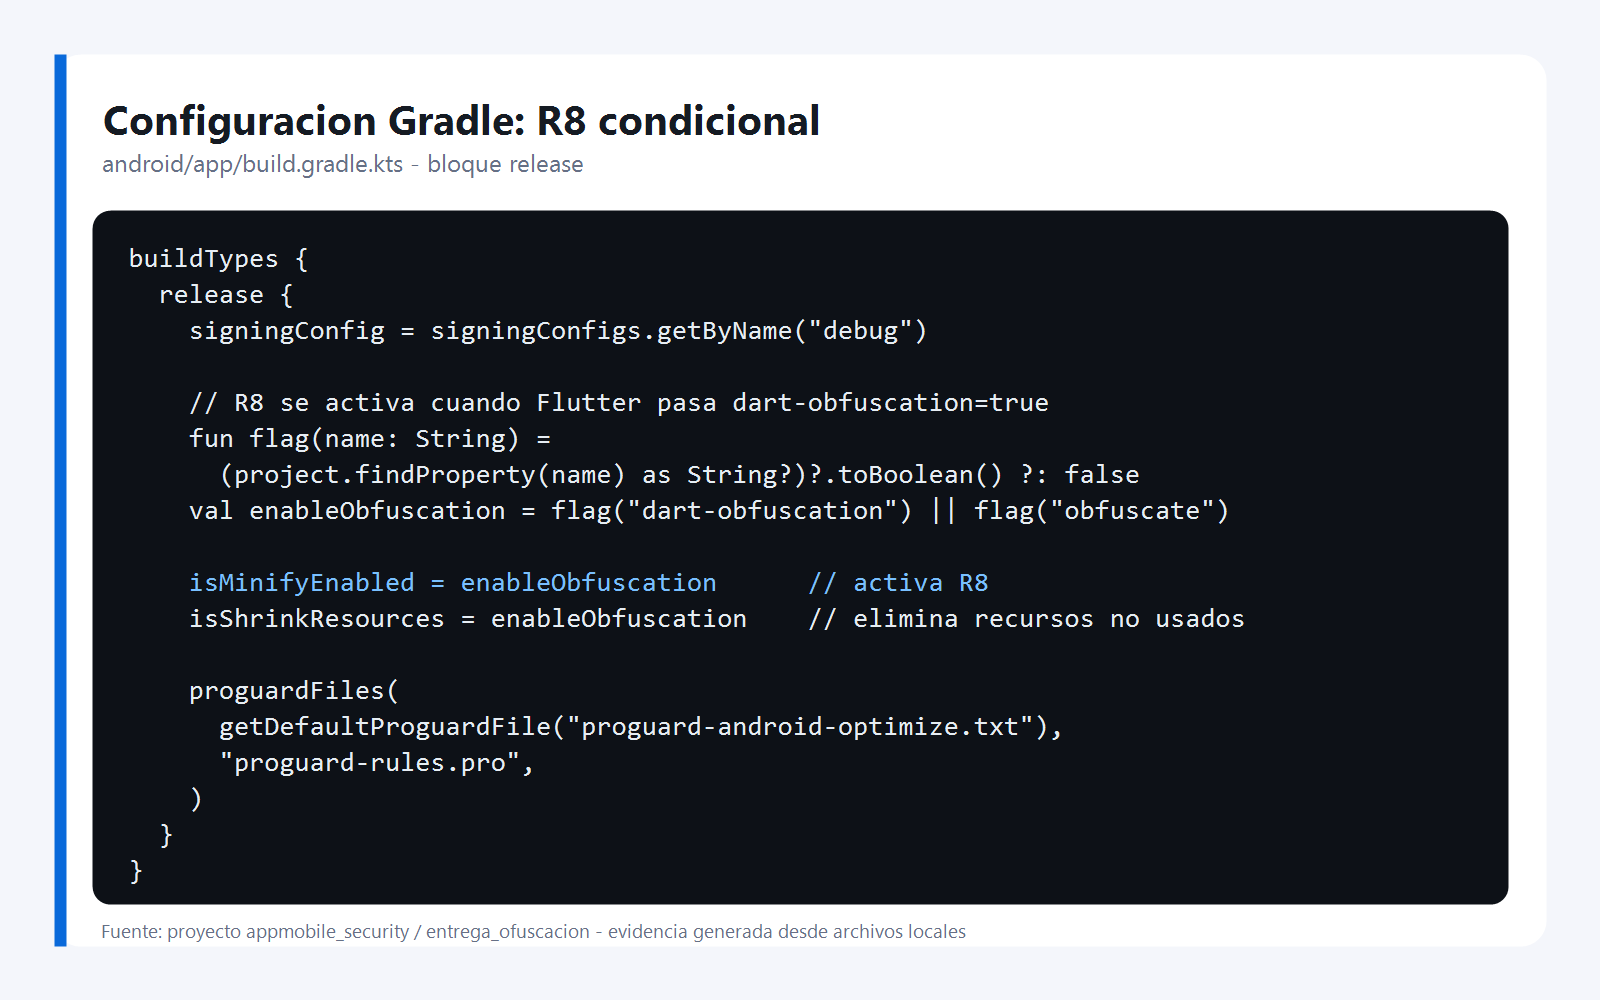
\includegraphics[width=0.95\linewidth]{capturas/01_gradle_config.png}
\caption{Configuración de \texttt{build.gradle.kts}: R8 se activa de forma
condicional cuando la compilación recibe \texttt{dart-obfuscation=true} o
\texttt{obfuscate=true}.}
\label{fig:cap-gradle}
\end{figure}

\begin{figure}[htbp]
\centering
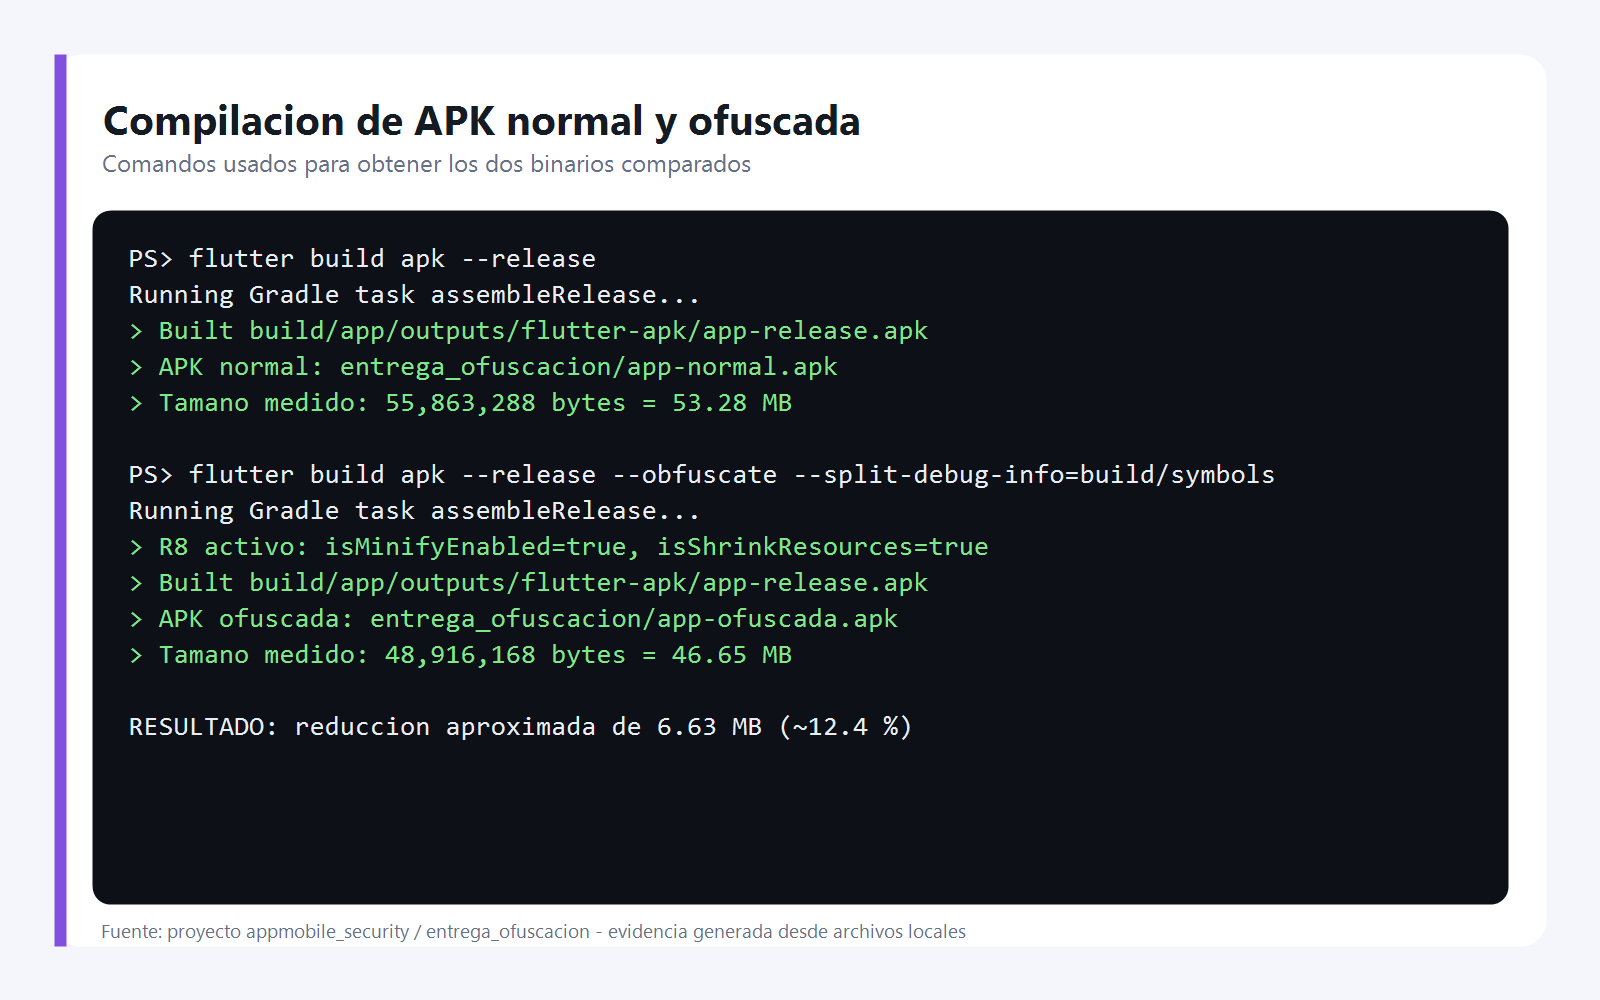
\includegraphics[width=0.95\linewidth]{capturas/02_build_output.png}
\caption{Comandos de compilación usados para generar la APK normal y la APK
ofuscada. La segunda versión activa \texttt{--obfuscate} y guarda la información
de depuración separada en \texttt{build/symbols}.}
\label{fig:cap-build}
\end{figure}

\begin{figure}[htbp]
\centering
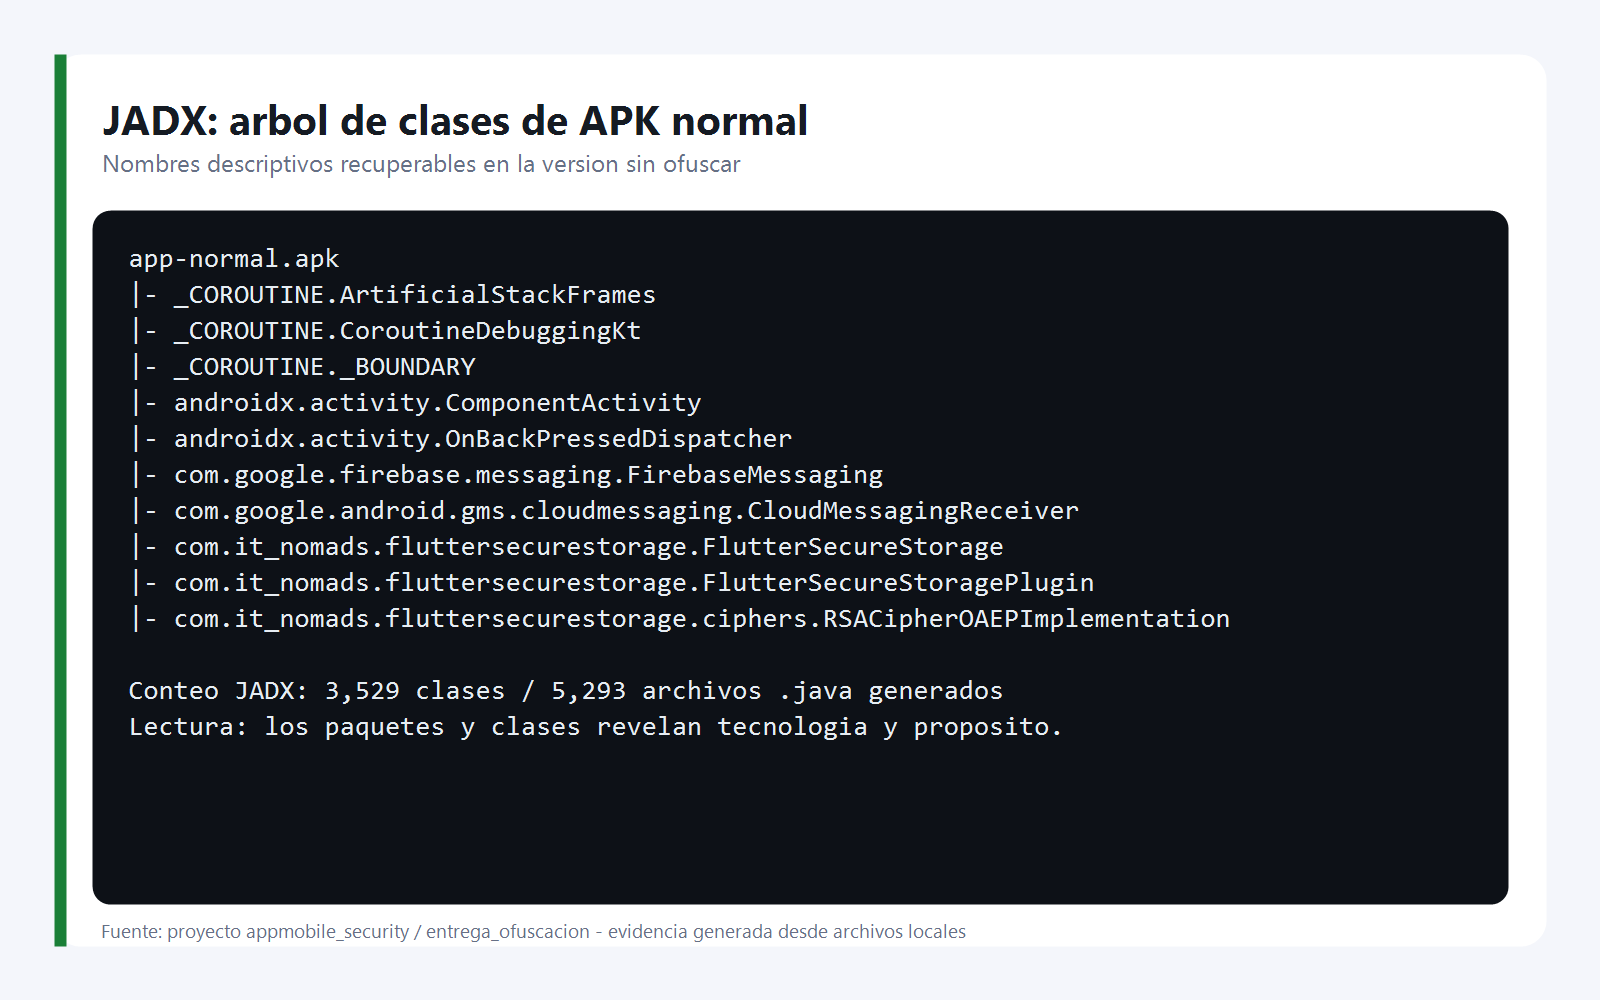
\includegraphics[width=0.95\linewidth]{capturas/03_jadx_normal.png}
\caption{Vista representativa del árbol de clases de la APK normal en JADX. Los
nombres de paquetes y clases son descriptivos, por lo que revelan tecnologías y
responsabilidades internas.}
\label{fig:cap-jadx-normal}
\end{figure}

\begin{figure}[htbp]
\centering
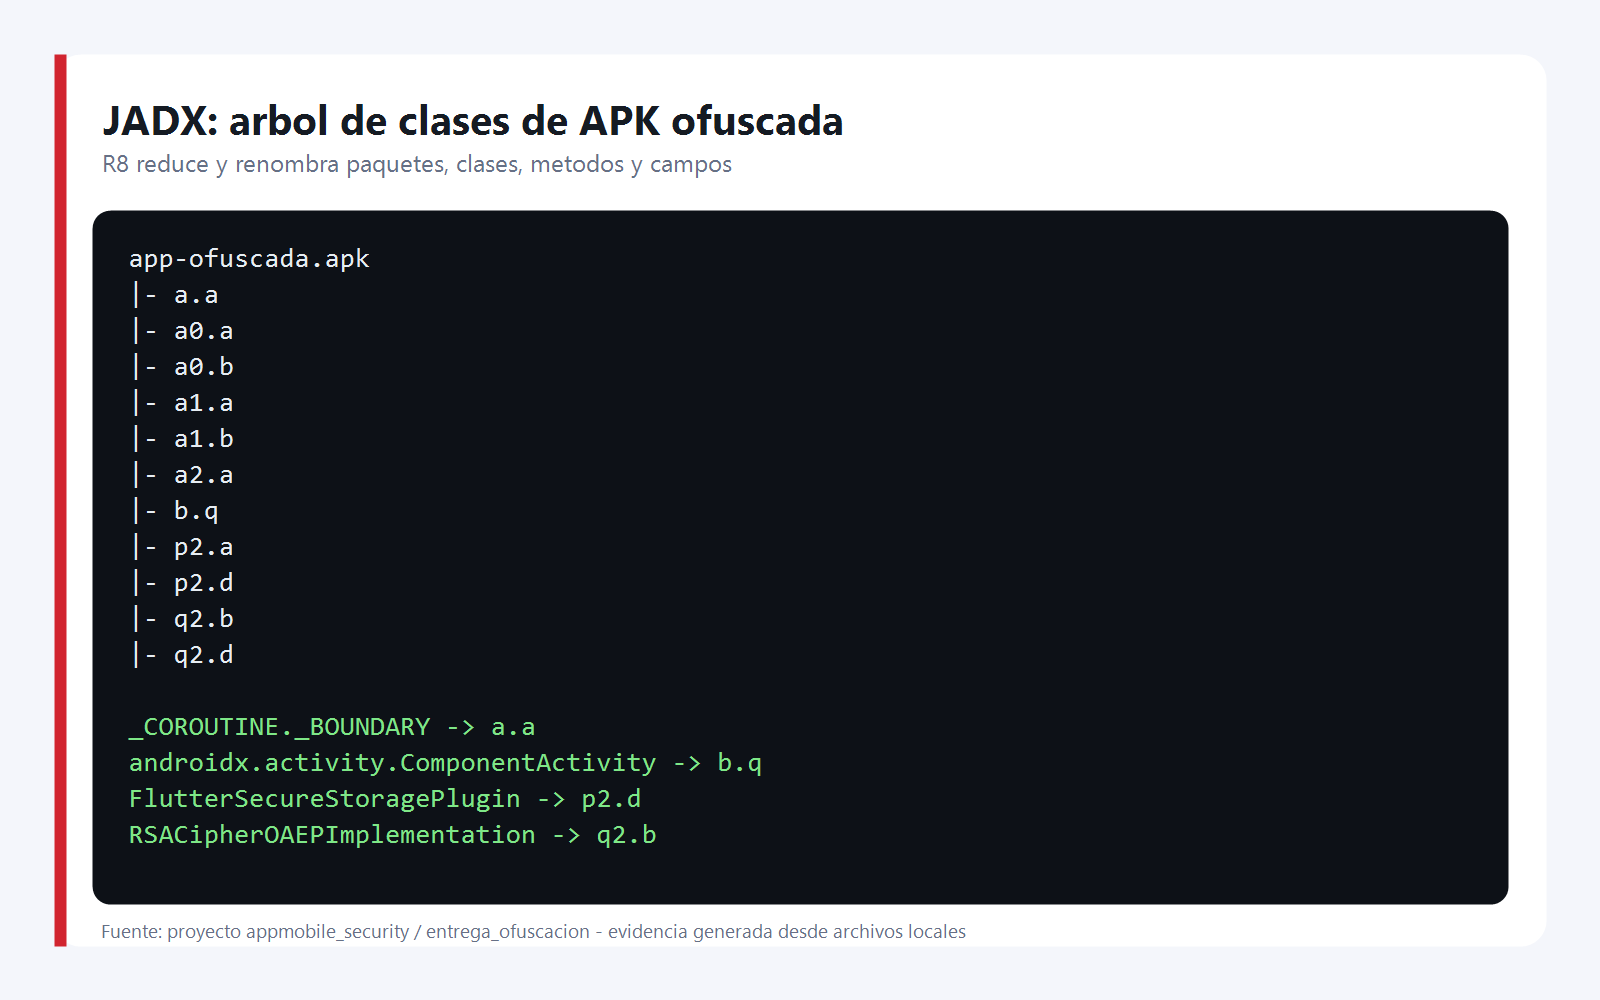
\includegraphics[width=0.95\linewidth]{capturas/04_jadx_ofuscada.png}
\caption{Vista representativa del árbol de clases de la APK ofuscada en JADX.
R8 reduce el número de clases y renombra elementos a identificadores cortos como
\texttt{a.a}, \texttt{b.q}, \texttt{p2.d} y \texttt{q2.b}.}
\label{fig:cap-jadx-ofuscada}
\end{figure}

\begin{figure}[htbp]
\centering
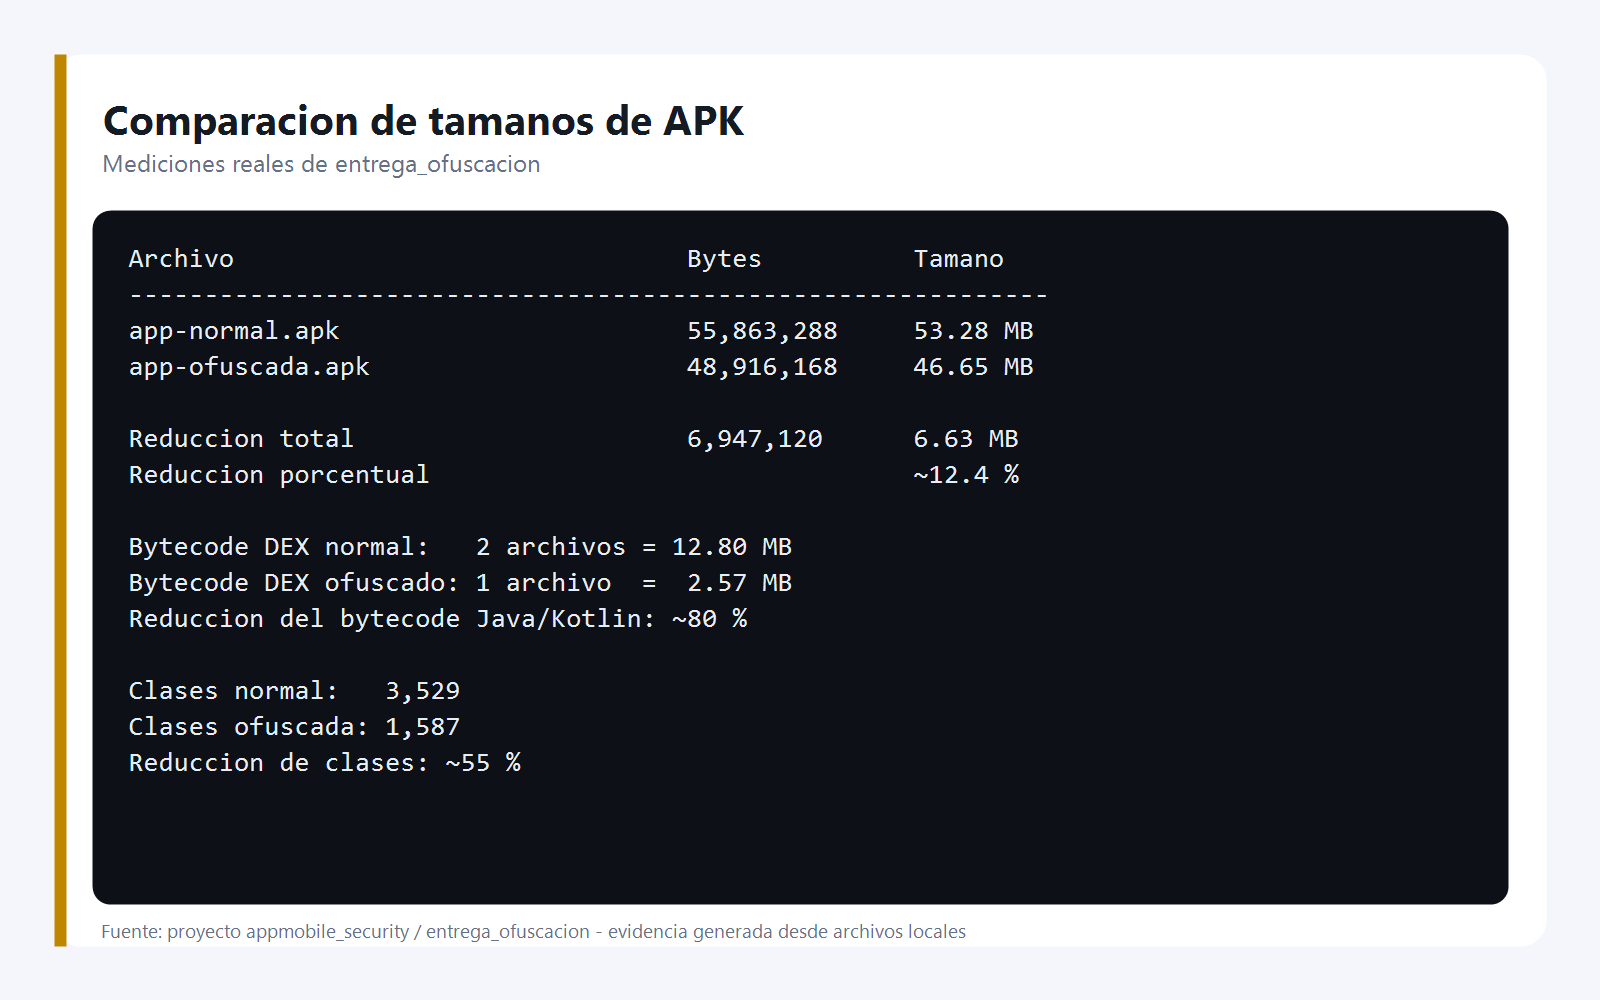
\includegraphics[width=0.95\linewidth]{capturas/05_tamanos.png}
\caption{Comparación de tamaños entre los dos APK generados. La versión
ofuscada reduce el tamaño total y, especialmente, el bytecode DEX de la capa
Java/Kotlin.}
\label{fig:cap-tamanos}
\end{figure}

\subsection{Análisis de los resultados}

La diferencia más evidente es \textbf{cualitativa}: en la versión normal, un
analista lee de inmediato nombres como \texttt{FlutterSecureStoragePlugin} o
\texttt{FirebaseMessagingPlugin}, lo que revela qué tecnologías usa la app y por
dónde fluyen los datos sensibles. En la versión ofuscada, esos nombres
desaparecen y el analista debe reconstruir el propósito de cada clase a partir
del comportamiento, lo que multiplica el esfuerzo.

En cuanto al \textbf{tamaño}, el \emph{shrinking} de R8 redujo el APK de
53.28~MB a 46.65~MB. El efecto más notable está en el \emph{bytecode}: los
\textbf{dos} archivos \texttt{.dex} de la versión normal (12.80~MB en total) se
redujeron a \textbf{uno} solo de 2.57~MB (cerca del 80\% menos), y el número de
clases bajó de 3\,529 a 1\,587 ($\approx 55\%$ menos). Es decir, la versión
ofuscada es \emph{más pequeña} pese a incorporar más protección, porque el
\emph{tree-shaking} eliminó todo el código no alcanzable. La capa Dart, al estar
compilada AOT, no cambia de tamaño de forma apreciable, pero \texttt{--obfuscate}
extrajo sus símbolos al mapa de \texttt{build/symbols} y los ocultó del binario.

% =====================================================================
%  5. CONCLUSIONES
% =====================================================================
\section{Conclusiones personales}

La práctica confirma que la ofuscación es una medida \textbf{necesaria pero no
suficiente}. Es necesaria porque su costo de implementación es bajísimo —apenas
una bandera de compilación y un archivo de reglas— y, a cambio, eleva de forma
considerable el esfuerzo que un atacante debe invertir para entender el código:
los nombres descriptivos desaparecen y la lógica deja de leerse «de un vistazo».
Para propiedad intelectual y para entorpecer el \emph{repackaging}, su valor es
real.

Sin embargo, la práctica también deja claro que la ofuscación \textbf{no
protege secretos}. Una cadena embebida (una clave de API, una URL) sigue estando
en el binario y puede recuperarse; lo único que cambia es el nombre de la
variable que la contiene. Por eso la conclusión es que la ofuscación debe
formar parte de una estrategia de \emph{defensa en profundidad}: secretos en el
servidor, almacenamiento cifrado, TLS con \emph{pinning}, validación del lado
servidor, anti-\emph{tampering} y detección de entornos no confiables. La
ofuscación encarece el ataque; las demás capas lo previenen.

% =====================================================================
%  6. PREGUNTAS DE REFLEXIÓN
% =====================================================================
\section{Preguntas de reflexión}

\subsection*{¿La ofuscación impide completamente la ingeniería inversa?}
No. La ofuscación \textbf{no impide} la ingeniería inversa; únicamente la
\emph{encarece}. El código sigue presente y ejecutable, de modo que un analista
con tiempo y herramientas (decompiladores, análisis dinámico con Frida,
depuradores) puede reconstruir el comportamiento. Lo que cambia es el
\emph{costo}: lo que sin ofuscación toma minutos, con ofuscación puede tomar
horas o días. Es una barrera disuasoria, no un muro infranqueable.

\subsection*{¿Qué información sigue siendo visible después de aplicar ofuscación?}
\begin{itemize}[leftmargin=1.4em]
  \item Las \textbf{cadenas literales} (\emph{strings}): claves, URL, mensajes,
        nombres de tablas; R8 no las cifra por defecto.
  \item El \texttt{AndroidManifest.xml}: permisos, \emph{activities},
        \emph{services} y \emph{providers}.
  \item Las \textbf{llamadas a la API del sistema y a bibliotecas} (p.ej.
        \texttt{android.security}, \texttt{HttpURLConnection}, Firebase), que
        revelan qué hace la app aunque los nombres propios estén ofuscados.
  \item Las clases conservadas por reglas \texttt{-keep} (Flutter, Firebase,
        \texttt{MainActivity}).
  \item Los \textbf{recursos}, \emph{assets} e imágenes.
  \item El comportamiento observable en ejecución (tráfico de red, archivos,
        valores en memoria) mediante análisis dinámico.
\end{itemize}

\subsection*{¿Qué riesgos existirían si una aplicación crítica se distribuye sin ofuscación?}
Una app crítica (banca, salud, pagos) sin ofuscación expone su lógica de negocio
y su estructura a cualquiera. Los riesgos concretos son: extracción inmediata de
secretos y \emph{endpoints}; identificación rápida de vulnerabilidades;
\textbf{evasión trivial} de controles del lado cliente (límites, validaciones,
detección de \emph{root}); \emph{repackaging} y troyanización con redistribución
maliciosa; clonación del producto; y un descenso drástico en el costo de un
ataque dirigido, ya que el atacante «lee» el diseño en lugar de inferirlo.

\subsection*{¿Qué otras medidas de seguridad deberían complementar la ofuscación?}
\begin{itemize}[leftmargin=1.4em]
  \item \textbf{Secretos del lado servidor} y tokens de corta duración; nunca
        \emph{hardcodear} claves.
  \item \textbf{Almacenamiento seguro}: Keystore/Keychain,
        \texttt{EncryptedSharedPreferences}.
  \item \textbf{TLS + \emph{certificate pinning}} para evitar
        \emph{man-in-the-middle}.
  \item \textbf{Validación del lado servidor} de toda regla de negocio.
  \item \textbf{Cifrado} de cadenas y datos sensibles.
  \item \textbf{Anti-\emph{tampering} / RASP}: detección de \emph{root},
        emulador, depuración USB, \emph{hooking}; verificación de integridad y
        de firma; \emph{Play Integrity API}.
  \item \textbf{Autenticación y autorización robustas} (OAuth2, MFA).
\end{itemize}
Este proyecto ya incorpora varias de ellas: almacenamiento cifrado, detección de
depuración USB, detección de \emph{Fake GPS} y \emph{wipe} remoto de datos
sensibles.

\subsection*{¿Es suficiente la ofuscación para proteger secretos, tokens o credenciales?}
\textbf{No, no es suficiente, y este es su límite más importante.} La ofuscación
renombra identificadores, pero \emph{no cifra los valores constantes}. Un token,
una clave de API o una URL escritos en el código quedan como cadenas literales
dentro del binario y se recuperan con un simple volcado de \emph{strings} o
abriendo el APK en JADX, sin importar que la variable que los contiene se llame
\texttt{a} en lugar de \texttt{apiKey}. Además, aunque el secreto estuviera
cifrado, la app necesita descifrarlo para usarlo, de modo que la clave de
descifrado también vive en el dispositivo y puede capturarse en tiempo de
ejecución. La regla práctica es: \textbf{todo secreto que llegue al dispositivo
debe considerarse comprometido}. Los secretos deben residir en el servidor; al
cliente solo deben llegar credenciales temporales, de alcance limitado y
revocables. La ofuscación protege la \emph{lógica}, no los \emph{secretos}.

% =====================================================================
%  REFERENCIAS
% =====================================================================
\section*{Referencias}
\addcontentsline{toc}{section}{Referencias}
\begin{itemize}[leftmargin=1.4em]
  \item Android Developers. \textit{Shrink, obfuscate, and optimize your app}
        (R8). \url{https://developer.android.com/build/shrink-code}
  \item Flutter. \textit{Obfuscating Dart code}.
        \url{https://docs.flutter.dev/deployment/obfuscate}
  \item Guardsquare. \textit{ProGuard / DexGuard manual}.
        \url{https://www.guardsquare.com/}
  \item OWASP. \textit{Mobile Application Security Verification Standard
        (MASVS)} y \textit{Mobile Security Testing Guide (MSTG)}.
        \url{https://owasp.org/www-project-mobile-app-security/}
  \item skylot. \textit{JADX — Dex to Java decompiler}.
        \url{https://github.com/skylot/jadx}
  \item iBotPeaches. \textit{Apktool}.
        \url{https://apktool.org/}
\end{itemize}

\end{document}
